\documentclass[a4paper,12pt,twoside]{ThesisStyle}
\usepackage[utf8]{inputenc}
\usepackage{thesis-style}
\usepackage{url}
\usepackage{booktabs}
\usepackage[table,xcdraw]{xcolor}
\usepackage{longtable}
\usepackage{lscape}
\usepackage{multirow}
\usepackage{subfig}

\begin{document}

\frontmatter

\pagenumbering{gobble}

\thispagestyle{empty}
\begin{table}[htb]
\centering
\begin{Large}
\resizebox{\textwidth}{!}{\begin{tabular}{ | l |}
 \hline
 \\

\includegraphics[scale=0.9]{imatges/logo_eps.png} \\
\centerline{\textbf{Master's Degree Thesis}}\\[1cm]
\hline
\\
\textbf{Degree}: Master in Data Science\\[0.7cm]
\hline
\\
\parbox{16cm}{\textbf{Title}: The Past and Present of Predictive Models for Anomaly Detection in Smart Cities: }
\\[0.5cm]
A Systematic Review
\\[0.7cm]
\hline
\\
\textbf{Document}: Summary\\[0.7cm]
\hline
\\
\textbf{Student}: Andrea Carolina Ramirez Moya\\[0.7cm]
\hline
\\
\textbf{Tutor}: Mateu Villaret Auselle\\
\textbf{Department}: Computer Science, Applied Mathematics and Statistics\\
\textbf{Area}: Languages and Computer Systems\\[0.7cm]
\\
\textbf{Co-Tutor}: Marc Comas Cufi\\
\textbf{Department}: Computer Science, Applied Mathematics and Statistics\\
\textbf{Area}: Statistics and Operations Research\\[0.7cm]
\hline
\\
\textbf{Call}: September 2023\\[0.7cm]
\hline

\end{tabular}}
\end{Large}
\end{table}

\newpage
\hypersetup{pageanchor=false}
\begin{titlepage}

% Upper part of the page

\includegraphics[scale=0.9]{imatges/logo_eps.png} \\[1cm]
\begin{center}
\textsc{\Large Master's Degree Thesis} \\[1cm]

% Title
\begin{spacing}{2}
\HRule \\
\textbf{\Huge The Past and Present of Predictive Models for Anomaly Detection in Smart Cities: A Systematic Review} \\
\HRule \\[0.5cm]
\end{spacing}

% Author and supervisor and other data
{
\large
\emph{Author:} \\
Andrea Carolina \textsc{Ramirez Moya} \\[1cm]
September 2023 \\[1cm]
Master in Data Science \\[1cm]
\emph{Tutors:} \\
Mateu \textsc{Villaret Auselle} \\
Marc \textsc{Comas Cufi} \\
}

\end{center}
\end{titlepage}
\hypersetup{pageanchor=true}

\titlepage

%\dominitoc


\pagenumbering{roman}

\chapter*{Abstract}
%\label{cap:resum}

Detecting anomalies in smart cities is a novel area that started being studied in the 21st century. This master's thesis aims to find the most accurate predictive models that can be explainable to scholars and industry stakeholders. With that goal in mind, a PRISMA 2020 for systematic literature reviews methodology is approached to review the papers that have been published in Emerald Insights, IEEE Xplore, Science Direct, and Web of Science with the concepts of Smart Cities, Data Science, and Predictive Models between 2000 and the first half of 2023. The findings show that the algorithms that have been studied the most are for classification, supervised machine learning. This thesis not only took into account the theoretical part, but also attempted addressing those techniques by forecasting the energy consumption in buildings in Barcelona, classifying if those outcomes were an anomaly, and finally clustering to find the consumption patterns. The deliverables are disclosed in a ObservableHQ notebook and a dashboard in Google Data Studio. 

\vspace{5mm} 
\textbf{Keywords}: Systematic Review, Predictive Models, XAI, Anomaly Detection, Smart Cities, Energy Consumption in buildings.

\vspace{10mm} 

La detecció d'anomalies en ciutats intel·ligents és una àrea nova que va començar a ser estudiada al segle XXI. Aquest treball de màster té com a objectiu trobar els models predictius més precisos que puguin ser explicables als acadèmics i a les parts interessades de la indústria. Amb aquest fi en ment, s'utilitza el PRISMA 2020 com metodologia per la revisió sistemàtica de la literatura dels treballs que han estat publicats en Emerald Insights, IEEE Xplore, Science Direct, i Web of Science amb els conceptes de Ciutats Intel·ligents, Ciència de Dades i Models Predictius entre 2000 i la primera meitat de 2023. Les troballes mostren que els algoritmes que més s'han estudiat són per a la classificació, l'aprenentatge automàtic supervisat. Aquesta tesi no només va tenir en compte la part teòrica, sinó que també va abordar aquestes tècniques mitjançant la predicció del consum d'energia en edificis de Barcelona, classificant si aquests resultats eren una anomalia, i finalment agrupant-se per trobar els patrons de consum. Els lliuraments es revelen en un quadern a ObservableHQ i un tauler de comandaments a Google Data Studio.

\vspace{5mm} 
\textbf{Paraules clau}: Revisió Sistemàtica, Models Predictius, Detecció d\'Anomalies, Ciutats Intel·ligents, Consum d'Energia en edificis, XAI.

\tableofcontents

\mainmatter

\chapter{Introduction}
\label{cap:intro}

\vspace{5mm} 

Cities are facing a digital transformation. Part of it comes from using technology to its advantage to ensure its citizens' safety and quality of life. Governments are seeking tools to predict and alert anomalies to make informed and optimal decisions in cases of emergency to take action and address those problems. However, one limitation is that those forecasting measures must be explainable to ensure transparency and clarity in communicating with stakeholders.

Explainable models give cities a clear and detailed account of how predictions are developing, allowing them to rely on alerts and take appropriate action to address problems detected in the public sector. Additionally, these models are easier to interpret and communicate to other stakeholders, such as citizens and department members, which can foster transparency and trust in local government.

While continuing to be fragmented and interdisciplinary, knowledge production is speeding up dramatically in the Machine Learning world. As a result, it is challenging to assess the amount of information in this field and remain on the leading edge of knowledge when selecting forecasting models. This research aimed to identify a series of predictive models that are optimal in detecting and, consequently, issuing alerts in the event of finding any anomaly in the data. In this way, it contributes significantly to improving the efficiency and effectiveness of public sector data management/governance, translating into better service and well-being for their citizens.

For those reasons, the aim for this master's thesis is to find the most accurate predictive models that can be explainable to academics and industry stakeholders by inspecting and critically assessing prior studies and scholarly writings related to predictive models for anomaly detection in smart cities. 

The questions this literature review wanted to answer were:

\begin{itemize}
  \item Which area of a city has been studied the most, and which areas are in need of development?
  \item Which predictive models are being used on anomaly detection in smart cities? Are those models using supervised or unsupervised machine learning techniques?
  \item Which databases of bibliographical references has the most resources?
\end{itemize}

In Chapter 2 of the thesis, the preliminaries of the concepts were explained to envision this study. In Chapter 3, the planning and methodology mapped the road to review the publications related to anomaly detection in smart cities. In Chapter 4, the state of the art portrays the past and present of this field within the literature found. In Chapter 5, the experimentation performed the anomaly detection models that were relevant to the reviewed authors. Chapter 6 shows the results from the evaluation of those approaches, and Chapter 7 concludes the project with some discussion and future work.

\chapter{Methodology}

This research created a solid foundation for current and future research by identifying, analyzing, and reporting patterns in 45 open-access papers. It provides a broader and more rigorous perspective regarding possible solutions and approaches to addressing this problem. It is accurate because it sought papers searched on Emerald Insights, IEEE Xplore, Science Direct, and Web of Science, in the category of Smart Cities, Data Science in the public sector, and Predictive Models in the twenty-first-century (2000-2023) by following the checklist provided by the “PRISMA 2020 explanation and elaboration: updated guidance and exemplars for reporting systematic reviews”~\cite{PRISMA2020}. 

All the decisions for the search strategy were written down on several tables to enable transparency for the criteria considered when selecting and classifying the papers, and the content analysis. It also followed the four-phase guidelines “to assess the quality of a literature review”~\cite{guidelinesLRSnyder2019} that include design, conduction, analysis, and writing the review.

A limitation found in this stage was the amount of papers published. Depending on the strategy approached, more than 1,000 papers would be needed to be reviewed. In view of this, the secondary concepts selected benefited the filtering, so the papers that contain at least one relevant keyword or term in their title. Finally, the papers were screened by keywords and abstract to ensure the studies were within this project's scope. 

Several studies were not relevant to this review since they are related to Blockchain, Cloud, Edge, and Fog Computing, Deep Learning, Reinforcement Learning, Adversarial Learning, and Federated Learning, which are out of the scope of explainable predictive modeling. 

To perform the content analysis, a \textit{Google Form} (\url{https://shorturl.at/akluK}) was created for the analysis, and interpretation of the studies. This tool works as a replicable method based on explicit criteria for downsizing large amounts of text into reduced content categories of the different publications. Using this tool it was more manageable to count the frequency of the keywords and concepts with a manifest focus in the scope of this study. 

The report on the review was performed in a chronological way. There is a brief summary of the history related to anomaly detection, and how the concept has evolved in the machine learning world. Then each concept is studied and portrayed by stating which authors used the same frameworks or different approaches in smart cities, data science and predictive models for anomaly detection.

Following those outcomes, with the CRISP-DM methodology, there was an experimentation section with the electricity consumption in Barcelona to model what the authors stated to forecast them and alert if the values are above or below the historic registers. 

The models that were appropriate to work were:
\begin{itemize}
  \item For forecasting purposes the SAX with SARIMA, or the Linear Regression,
  \item for classification effects the RF. Since on other fields the KNN, SVM and XGBoost had high accuracy scores they will be also be taken into account,
  \item for clustering outcomes the K-Means.
\end{itemize}

\sloppy The data was accessed on the Barcelona's open data website (\url{https://opendata-ajuntament.barcelona.cat/data/en/dataset/consum-electricitat-bcn}). By the time of study, the historical data was from January 2019 until March 2023. 

The records didn't come as a time series but as aggregation windows in 5 categories: from 00:00:00 to 05:59:59, from 06:00:00 to 11:59:59, from 12:00:00 to 17:59:59, from 18:00:00 to 23:59:59, and not specified. Due to computational performance issues, only the nighttime windows were used as it is when they should be idle, and an anomaly could be more feasibly detected, and only in the Gothic borough since this area houses the government of the city.

\begin{figure}[hbt]
\centering
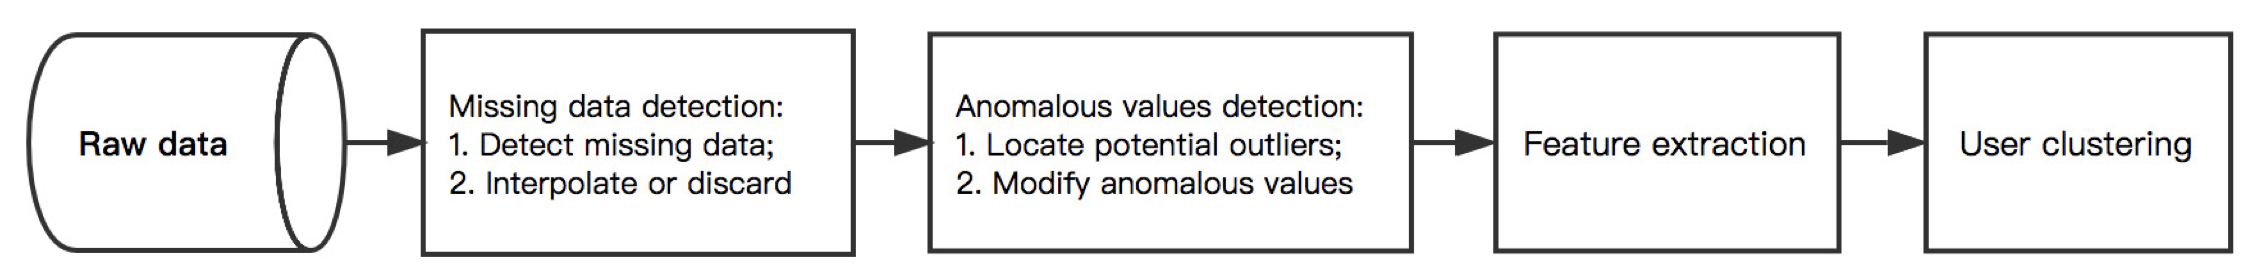
\includegraphics[width=13 cm]{imatges/dataProcessing.png}
\caption{\label{fig:dataProcessing} Data processing procedure proposed by~\cite{du2019clustering}.}
\end{figure}

The dataset for \textit{electricity consumption in Barcelona} had a similar structure to the Swedish city's heat meter records of buildings used by~\cite{du2019clustering}. In this publication, they propose a data processing procedure (figure~\ref{fig:dataProcessing}) where they first pre-process the data, then detect the anomalies, extract some features, and then cluster the users' behavior, all based on heat consumption. 

The data analysis (processing for modeling) part used Apache Spark's built-in features from its library \textit{pyspark}, as mentioned by~\cite{liu2018scalable}. However, for modeling purposes, the library \textit{pandas} was utilized for querying the algorithms.



\chapter{Results}

The reference database that had the most papers to review was Science Direct (64\%), followed by Web of Science (20\%), IEEE (13\%), and last Emerald (2\%). 

With in the energy field, the were found three categories that explain the area by the consumption, efficiency, and the load of energy.

Energy consumption was the most studied. Some authors that have talked regarding classification methods are ~\cite{cerquitelli2017predicting} and~\cite{leiria2021using}; and clustering are~\cite{fonseca2017unsupervised} and~\cite{du2019clustering}.

As a result of so many record reductions due to computational resources, when testing the training set, the accuracy showed an overfitted outcome from KFold Cross-Validation; with 99.45\% in the KNN and 100.0\% in the SVM, either linear or Radial Basis Function.

In spite of this, the models on the forecasted data were conclusive. The models had a similar accuracy. Nonetheless, the KNN model was more accurate (88.09\%) and had fewer mislabeled points than the others (10 out of 84). Still, there is a lot of room for improvement as the predictions are labeled as \textit{Average} non-average records which could be harmful.

The most important features are the average type (below, above and average) and the consumption value despite having more attributes like the month or the activities that were happening that day.

For this dataset, the optimal number of clusters is 2 with a prediction strength of 1.0, even though there is a turning like an elbow between k=2 and k=3. 

The final outcome of this project is to spread the word and make it easier for people in the academia and the industry to gain more knowledge of detecting anomalies in smart cities with predictive models. A way to visualize the results found is by presenting a deliverable.

To use the resources learned throughout the master's degree, an \textit{ObervableHQ} was created with systematic review that can be found in: \url{https://observablehq.com/@andreaudg/anomaly-detection-lit-rev}.

Then to expose the experimentation results a dashboard was created to grasp the energy consumption in service buildings in the Gothic borough at night-time. It can be found in \url{https://lookerstudio.google.com/s/j_93RGA8KF0}.


\chapter{Conclusions and Future work}
\label{cap:concl}

To answer the initial research questions, 
\begin{itemize}
  \item \textit{Which area of a city has been studied the most, and which areas are in need of development?}
\end{itemize}
The city area studied the most is \textbf{transportation} which follows the trend within the scope of anomaly detection literature. It was closely followed by cybersecurity and energy. The areas that need development are the environment, people's mobility, and structures. There were no studies related to the living and security of the people.
\begin{itemize}
  \item \textit{Which predictive models are being used on anomaly detection in smart cities? Are those models using supervised or unsupervised ML techniques?}
\end{itemize}
The predictive models used the most to detect anomalies in smart cities are \textbf{classification}, which are \textbf{supervised ML techniques} such as RF, XGBoost, SVM, and KNN. However, some studies performed unsupervised clustering using K-Means and DBSCAN, depending on the anomaly type.
\begin{itemize}
  \item \textit{Which databases of bibliographical references has the most resources?}
\end{itemize}
The bibliographical reference database with the broader scope of published open access papers is \textbf{Science Direct}. \textit{IEEE} has a smaller section of conference papers instead of journals.

Despite referencing key ideas, several disqualified papers on the bibliographical reference databases did so because they correspond to a more theoretical than practical area. They emphasized more on potential solutions and upcoming difficulties. They discuss the possibilities in the area, notably the health sector and cybersecurity, but leave enormous room for future research. They have been used as case studies thus far, but there have yet to be any outcomes in anomaly detection. 

Throughout the development of the systematic literature review, I found limitations in the discussion of some topics, as they were mentioned in a latent way and just hinted at the subject. As a result, this opens an door for future research on data governance and the people's security in smart cities. In the future, the systematic review could be carried out using NLP (Natural Language Processing) tools to be able to address more publications. In this way, it would be more feasible to use search strategies that include more than 2.000 papers.

Papers are stuck in the analysis phase of the data collection and what happens after the models have predicted the anomalies is absent. They also do not present a data mining/acquisition approach; their smart data models are juxtaposed to data architecture, blending it into one topic.

The experimentation utilized 130.872 records, as there were initially more than one million records. For future work, more robust performance with more than 2GB of memory capacity is needed for the models to be trained in all the types of buildings in the city, in all boroughs, and at all times of the day, not only in the overnight period (from 18h to 5h), selected to lower the dataset size.

The operations part of ML and how these types of models can be brought to production can also be addressed.

\backmatter

\bibliographystyle{ThesisStyleBreakable}
\bibliography{biblio}

%\chapter{Appendix}
%\label{cap:appendix1}


%\printnomenclature

\end{document}
